\documentclass[12pt, a4paper, twoside, openright]{book}

\usepackage{vuwthesis} % sets up some local things, mostly the front page

\usepackage{palatino} % sets palatino as the default font

\usepackage{url} % for typesetting urls

\usepackage{graphicx}
\usepackage{amsmath}
\usepackage{amssymb}
\usepackage{hyperref}
\DeclareUnicodeCharacter{2212}{-}
\providecommand{\tightlist}{%
  \setlength{\itemsep}{0pt}\setlength{\parskip}{0pt}}

%\renewcommand{\baselinestretch}{1.00}


\begin{document}

\frontmatter
% Book style knows about front matter
% Report style doesn't so you need to set roman numbering etc yourself :-(

%%%%%%%%%%%%%%%%%%%%%%%%%%%%%%%%%%%%%%%%%%%%%%%%%%%%%%%

\title{ABSTRACTION FOR EFFICIENT REINFORCEMENT LEARNING}
\author{Alexander Telfar}

\subject{Computer Science}
\abstract{An abstract of fewer than 500 words must be included.}
% Books don't normally have abstracts, and this is a bit of a hack

% Uncomment the appropriate degree
% \phd
\mscthesisonly
% \mscwithhonours
%\mscbothparts
% \otherdegree{DEGREE OR DIPLOMA NAME}



%%%%%%%%%%%%%%%%%%%%%%%%%%%%%%%%%%%%%%%%%%%%%%%%%%%%%%%




\maketitle

\chapter*{Acknowledgments}\label{C:ack}

Mostly, I would like to thank my advisers: Will Browne, for supporting my work and giving me the freedom to explore my interests.
And Brendan McCane for some timely feedback.

I would like also to thank Marcus Frean and Stephen Marsland for providing a

And finally, I would like to thank my family.

{\color{red}who am i being paid by again!? forestry something something. should thank them!?}

% also thankful for ...? arms, eyes, health, purpose, money, safety, ... a long list.


\tableofcontents


%%%%%%%%%%%%%%%%%%%%%%%%%%%%%%%%%%%%%%%%%%%%%%%%%%%%%%%

% book style knows about mainmatter
% if you are using report style you will have to rest page numbering etc.
\mainmatter

%%%%%%%%%%%%%%%%%%%%%%%%%%%%%%%%%%%%%%%%%%%%%%%%%%%%%%%

% individual chapters included here

\chapter{Introduction}\label{C:intro}

% RL is inefficient
Reinforcement learning has an efficiency problem: AlphaGo \cite{Silver2016a}, the Go
playing AI that beat world champion Lee Sedol, needed 1.28 million games, with
extra supervision from another 29.4 million positions, while learning with 50 GPUs.
Libratus \cite{Brown2018b}, the poker playing AI that beat a table of professionals,
constructed its poker-playing strategy over 15 million processor-core-hours.
OpenAI Five \cite{Berner2019}, the Dota 2 playing AI that beat OG, the winners of The International 8 and 9, was
trained over 10 months, at its peak, collected 900 years of experience per day using
128,000 CPUs and 256 GPUs.

\begin{displayquote}
\textit{Is reinforcement learning fundamentally inefficient, or can we do better?}
\end{displayquote}


\section{Motivation of this thesis}

Abstraction is about preserving essential structure and discarding inessential details.
We want to apply abstraction to reinforcement learning in the hope of building more efficient reinforcement learners.

\begin{displayquote}
\textit{By throwing away inessential details, there is less to compute. \newline
By throwing away inessential details, we don't need to explore them. \newline
By throwing away inessential details, we reduce the variance of our \newline
observations (allowing quicker learning).}
\end{displayquote}

% 1) Abstractions appear to essential for intelligent behaviour (ref some psyc / neuro paper?!).
%
% 2) Dimensionality reduction is not enough. Want to be able to preserve the important structure.
%
% % What strategies are there to improve the efficiency of RL?
%
% %  research question goes here!

The main goal of this thesis is to understand:

\begin{displayquote}
\textit{to what extent can abstractions increase the efficiency of reinforcement learning?}
\end{displayquote}

\section{Overview}

Given the goal above, we pick Markov Decision Problems as our setting for studying abstractions\footnotemark[43] and give a slightly non-standard, but general introduction to them, see section \ref{mdps}.
Then we explore abstractions and existing theory for understanding abstraction and attempt to organise it in to a clearer framework, see section \ref{abstraction-rl}.
Next, we analyse an existing method of abstraction for efficient control and find that it does not work in general, see section \ref{solveable-abstractions}.
Finally, we build an abstraction using symmetries, see section \ref{symmetric-abstractions}.

\footnotetext[34]{In general, when we state abstractions, we mean abstractions for reinforcement learning.}

\section{Contributions}

In this thesis, we;

\begin{itemize}
  \tightlist
  \item Construct a family of similarity measures for building abstractions for RL.
  \item Review the fields ability to evaluate abstractions.
  \item Clarify that a well cited method of abstraction doesn't work in general. \ref{lmdp-validation}
  \item Build a Thompson sampler that exploits the knowledge of a symmetry to achieve more efficient learning \ref{thompson-sampling} {\color{red}WIP}
  \item Explore methods of discovering symmetries and a complexity measure \ref{????} {\color{red}WIP}
  \item Generalise the notion of MDP homomorphism to temporal abstractions \ref{temporal-abstraction} {\color{red}WIP}
  \item Explore a new task for understanding a learners ability to generalise \ref{action-space-experiments}
  \item We explore the iteration complexity, effect of discounting, and the density of the Value functional polytope. \ref{polytope-extras}
  \item Provide a way to visualise the dynamics of learning an MDP in higher dimensions \ref{graph-vis}. It's utility is unclear.
  \item Formulate a type of model based learner \ref{model-iteration}, which has some serious, but potentially solvable, issues with larger problems.
\end{itemize}

% \chapter{Markov Decision Problems}

Reinforcement learning (RL) refers to the set of solutions to a type of problem.
This general, reinforcement learning, problem, has two main properties;
\textit{"trial-and-error search and delayed rewards"} \cite{Sutton2018}.

Unlike supervised learning, which gives the learner feedback (\textit{Student: "I think that digit
is a 5". Teacher: "No, it's a 6"}), in RL the learner only receives evaluations (\textit{Student: "I think
that digit is a 5". Teacher: "No."}). This means the student needs to explore the possible answers via some trial-and-error search.
(\textit{Student: "Is it a 4?". Teacher: "No." Student: "How about a 0?". Teacher: "No." ... Student: "A 6?". Teacher: "Yes."})

Ontop of terse teachers, many actions may be taken before any evaluation is received, thus requiring credit to be assigned to past actions,
(\textit{Student: "Is it a 4? How about a 0? A 6? Maybe a 7?". ... Teacher: "No".})
often leaving the learner wondering: "what did I do to deserve this?" (see
\href{https://www.youtube.com/watch?v=Qv4H81gEGDQ}{pigeon superstition} for an amusing
example of credit assignment gone wrong \cite{Box1997}).

% Your teaher might only give you evaluations for sequences of actions, rather than individual actions.
% Thus you are left with trying to infer how these sequence evaluations tells you about which actions you should take.

\vspace{5mm}

The above definition of reinforcement learning is quite general. There are many
different dimensions to problems that require trial-and-error search and give
delayed rewards. For example we could make a RL problem that is;

\begin{itemize}
\tightlist
\item
  Observable or un-observable \cite{Kaelbling1998}
\item
  Deterministic or stochastic \cite{Putterman2015}
\item
  Synchronous or asynchronous \cite{Bertsekas1995}
\item
  Terminating or infinite \cite{Putterman2015}
\item
  Discrete versus continuous \cite{Bertsekas1995}
\item
  Given knowledge of the underlying model  or not\cite{Sutton1991}
\end{itemize}

\begin{displayquote}
  \textit{But, which setting should we study?}
\end{displayquote}

\begin{displayquote}
  A better question might be: \textit{What is the simplest setting we can
  consider that still poses an interesting challenge to the ML and / or RL communities?}
\end{displayquote}

Markov decision problems (MDPs) appear to be a good candidate. Let's go through some definitions so we an more clearly understand how they can be used as a
simple setting to analyse RL.

Formally, a MDP, which is a type of sequential decision problem, is defined
as a tuple, $\{\mathcal S, \mathcal A, P,r, \gamma, d_0\}$.
Where $S$ is the set of possible states (\textit{for example arrangements of chess pieces}),
$A$ is the set of actions (\textit{the different possible moves, left,
right, diagonal, L-shaped step, ...}),  $P: S \times A \to \Delta(S)$\footnotemark[16]
is the transition function which describes how the environment acts in response
to the current state and to actions (\textit{You play pawn to pawn to D4, in response your
opponent moves, knight to D4, taking your pawn.}). Next is the reward function, $r: S\times A \to \mathbb R$,
(\textit{whether you won (+1) or lost (-1) the game }).
Lastly, the policy, $\pi: S \to \Delta(A)$, is what the learner gets to choose, aka the learners strategy.
It decides which action to take in different states.

\footnotetext[16]{The notation $\Delta(S)$ represents a distribution over S.}

\vspace{5mm}

The objective when solving a MDP is to find a policy
that maximises the expected cumulative discounted reward $V^{\pi}$ (aka the value). This
can be written as, maximising the expected return.

\begin{align*}
V^{\pi} &= \mathop{\mathbb E}_{\zeta \sim D(\pi, \tau)} [R(\zeta)] \\
\pi^{* } &= \mathop{\text{max}}_{\pi}V^{\pi}
\end{align*}


Where, $d_0$ is the initial state distribution, $\zeta$ collects the $(s_t, a_t, r_t)$ triples of a game (aka trajectory or rollout) \footnotemark[17],
$R(\zeta) =\sum_{t=0}^H \gamma^t \zeta^r_t$ is cumulative discounted reward (aka the 'return' of a single game), and $D$ is the probability of a trajectory under the chosen policy and MDP.

\footnotetext[17]{We allow $\zeta$ to be indexed by time and $\{s, a, r\}$. For example; $\zeta_t^s=s_t$.}

\begin{align}
\zeta &= \{(s_t, a_t, r_t) : t \in [0, H]\} \tag{trajectory} \\
D(\zeta, \pi, \tau, d_0) &= d_0(\zeta^s_0) \prod_{t=1}^{\infty} \pi(\zeta^a_t|\zeta^s_t) \tau(\zeta^s_{t+1}|\zeta^s_t, \zeta^a_t) \tag{p($\zeta$)}
\end{align}

% If we wanted we could pick our actions before we make observations,
% reducing the search space to only \(|A| \times T\). But this is a bad idea\ldots{} example.

You can find examples of some simple MDPs in \ref{MDP-examples}.

\section{Sequential decision problems}

A general intuition for the problem of solving a sequential decision problem is: actions (aka decisions) are made
sequentially (\textit{e.g. first we put on our socks then we put on our shoes}).
These actions need to be conditioned on the current state of the world (\textit{e.g. It is morning and time to go to work.}).
The goal is to take actions that achieve higher rewards (\textit{e.g. Lying in bed is quite rewarding...}). While instantaneous
rewards are good, we really care about long term cumulative rewards (\textit{e.g. Having a job and thus being able to afford a bed is more rewarding.}).

% Maze with pendulums / doors. When moving through the maze, you must
% swing the pendulums. In the future you must avoid being hit. (maybe make
% a picture of this?) also, is there a more general way to think about it?

\begin{displayquote}
  \textit{What does the M in MDP really mean?}
\end{displayquote}

When we say a decision problem is Markovian, we mean that the transition
function generates a Markov chain \cite{Markov2006}. The next transition step depends only
on the current state and action. It is invariant to any and all histories that do not
change the current state. \footnotemark[18]

\footnotetext[18]{Or another way of saying the same thing, there is no hidden state
that effects future transitions.}

This is not to say that past actions do not effect the future. Rather,
it is a special type of dependence on the past. Where the dependence is
totally described by changes to the state, $s\in S$.

We can return to chess for an example: in chess there are no hidden pieces, or
private knowledge about the current state. I know everything there is to know.

% Can easily make a sequence Markovian by adding information. E.g. time

\section{Solving a MDP}

\begin{displayquote}
  \textit{What does it mean to solve a MDP?}
\end{displayquote}

A MDP is considered solved when we have found the 'optimal' policy. As above,
the 'optimal' policy is the policy that gives the highest expected return (value).
This means that;

\begin{align*}
\pi^{*} : \;\; V^{\pi^* }(s) \ge V^{\pi}(s) \quad \forall \pi\in \Pi \;\;\forall s\in S\\
\end{align*}

Which is implied by our earlier definition, but the optimal policy also has some other properties of note.\cite{Bertsekas1996}

\begin{itemize}
\tightlist
  \item it always exists,
  \item it is deterministic, {}
  \item it is unique, or are there many optimal policies?{\color{red}unsure about this}
\end{itemize}

{\color{red}do I need to explain these?}

\subsection{The Bellman Equations}

{\color{red}how to intro / motivate bellman and TD??}

The expected return (value) can also be rewritten in a recursive manner,
which is known as the Bellman equation.

\begin{align*}
Q^{\pi}(s, a) &= r(s, a) + \gamma \mathop{\mathbb E}_{s' \sim P(\cdot|s, a)} [V(s')] \label{eq:bellman-eqn}\tag{Bellman equation}\\
V^{\pi}(s) &= \mathop{\mathbb E}_{a \sim \pi(\cdot|s)} [Q^{\pi}(s, a)]
\end{align*}

The formulation suggests a potential way to solve a MDP, through generalise policy iteration.
Pick a policy randomly, estimate its value, apply the Bellman operator, to get state-action values.
Construct a new policy by acting greedily with resepct to the state-action value. Repeat.

\begin{align*}
\pi(a| s) &= \mathop{\text{argmax}}_a Q(s, a) \label{eq:greedy}\tag{greedy}\\
\end{align*}

% \begin{align}
% T(V) &= \mathop{\text{max}}_a \big[r + \gamma PV\big] \\
% \end{align}

\subsection{Complexity}

\begin{displayquote}
  \textit{How hard is it to find the optimal policy?}
\end{displayquote}

% Insert lower bound and some intution
The complexity of estimating the value of a state-action under the optimal policy, ie solving the Bellman optimality
equation, can be glimpsed if we unroll its recursive definition.
Here we can see a series of nested maximisation problems, where the former
maximisation problems are conditional on the results of the latter maximisation problems.

\begin{align*}
Q^{\pi}(s_0, a_0) = r(s_0, a_0) &+ \gamma \mathop{\text{max}}_{a_1} \mathop{\mathbb E}_{s_1\sim p(\cdot | s_0, a_0)} \Bigg[ \\
r(s_1, a_1)  &+ \gamma \mathop{\text{max}}_{a_2} \mathop{\mathbb E}_{s_2\sim p(\cdot | s_1, a_1)} \bigg[\\
r(s_2, a_2)  &+ \gamma \mathop{\text{max}}_{a_3} \mathop{\mathbb E}_{s_3\sim p(\cdot | s_2, a_2)} \Big[
\dots \Big] \bigg] \Bigg]
\end{align*}

% {\color{red}TODO add some complexity bounds}

For the final maximisation problem we need to find the best action ($|A|$) for each potential final state we might be in ($|S|$).
Then we need to do this again for each maximisation problem (of which there are $|S|$).
So the computational complexity is $\mathcal O(|S|^2|A|)$.

\section{A tabular representation of MDPs}

Back to constructing a simple RL setting.

Imagine a MDP that can be described with tables (aka arrays). A table of
three dimensions can describe the transition probabilities, $P[s_{t+1}, s_t, a_t]$,
and a table of two dimensions can describe the rewards, $r[s_t, a_t]$: the
states and actions act as indexes to locations in the tables.
Let's formally define our tabular MDP. \footnotemark[23]

\footnotetext[23]{It should be noted that this tabular MDP setting ignores an important
aspect of RL: exploration, estimation error.}

\begin{align}
\mathcal M &= \{S, A, P, r, \gamma\}\; \tag{the MDP}\\
S &= [0:n-1] \tag{the state space}\\
A &= [0:m-1] \tag{the action space}\\
P &\in [0,1]^{n\times n \times m}, \;\;\forall j, k : \sum_i P[i, j, k] = 1 \tag{the transition fn}\\
r &\in \mathbb R^{n\times m} \tag{the reward fn}
\end{align}

A result of this formulation is that we concisely write and solve the \eqref{eq:bellman-eqn}. \footnotemark[0]

\footnotetext[0]{Note that the ability to solve the Bellman equation analytically does not allow
us to solve for the optimal policy analytically.}

\begin{align}
V &= r_{\pi} + \gamma P_{\pi} V \tag{tabular Bellman eqn}\\
V &= (I-\gamma P_{\pi})^{-1}r_{\pi}  \label{eq:value-functional}\tag{Value functional}
\end{align}

The values are written as a vector, $V \in \mathbb R^n$.
The reward under a given policy is written $r_{\pi}[s, a] = \pi[s, a] r[s, a]$.
And the transitions under a given policy is written $P_{\pi}[s', s] = \sum_a P[s', s, a]\pi[s, a]$.

An alternative derivation of the value functional, which is more verbose and more enlightening, can be found in \ref{vf-neumann}.

\begin{displayquote}
\textit{But why is the tabular MDP considered 'simple' enough?}
\end{displayquote}

Consider a MDP with deterministic actions, where $P(s_{t+1}|s_t, a_t) \in \{ 0, 1\}$.
This RL problem can be efficiently solved by non-statistical
methods: dynamic programming and related planning techniques \cite{Bertsekas1995}.

Rather, a MDP with stochastic actions, $P(s_{t+1}|s_t, a_t) \in [0, 1]$,
seems to retain much of the complexity we care about: this setting does not allow
efficient solutions via dynamic programming. And it can be approached with algorithms
that are used for state-of-the-art deep RL such as;
policy gradients \cite{Schulman2015a} and Q-learning \cite{Mnih2015}.

% \chapter{Related work}

How do the topics considered in this thesis relate to the work done in the wider scientific community and to society? Which work uses similar tools, which works build on the same foundations, which works have the same goals? How will this help? What can it be used for?

Decision theory (economics and psychology), ...?
Control theory

\section{Search spaces}


Recently there has been work investigating the properties of overparameterised search spaces.
Many \cite{Arora2018} (and others?!?!?) claim that overparameterisation yeilds acceleration, however,
their explanation of the acceleration is not entirely convincing.

\cite{Arora2018}'s proofs ...??


\section{Abstraction}

\hypertarget{representation-learning-and-abstraction}{%
\subsection{Representation learning and abstraction}\label{representation-learning-and-abstraction}}

The goal is to find a representation that decomposes knowledge into its parts.

Another way to frame this is: trying to find the basis with the right
properties.

\begin{itemize}
\tightlist
\item
  sparsity,
\item
  independence,
\item
  multi scale,
\item
  locality/connectedness
\item
  ???
\end{itemize}


Types of abstraction for RL. Abstraction for efficient;

\begin{itemize}
\tightlist
\item
  exploration, Learning latent state representation for speeding up exploration \cite{Vezzani2019}
\item
  optimal control,
\item
  ???,
\end{itemize}

Unsupervised State Representation Learning in Atari  \cite{Anand2019}
State Aggregation Learning from Markov Transition Data  !!!\cite{Duan2018}

\subsection{Linear RL}

Recently there have been a few other attempts to exploit linearity for RL.
\cite{Pires2016} factored

\cite{Wang} Reward and transitions are a linear function of features of a state-action pair.

Levine et al. \cite{Levine2019} build a latent representation such that the transition fn (in the latent space) is approximately linear. This allows ...

These attempts all focus on linearity in the transition function...

\subsection{Heirarchical reinforcement learning}

What is HRL? Really it is just temporal abstraction, using a heirarchy.

As far as I know, there are three main apporaches to HRL.
Equip an agent with options, learning to generate sub goals, pretrained low level policies, .


Between MDPs and Semi-MDPs \cite{RichardS.SuttonaDoinaPrecupb1998}
Reinforcement learning with structured hierarchical grammar representations of actions  \cite{Christodoulou2019}  !!! theory for this tho?!
Latent Space Policies for Hierarchical Reinforcement Learning \cite{Haarnoja}

Two main approaches. Subgoals and options. To achieve temporal abstraction.

- Does it help?
- Why does it help?
- ?

We don't really have a principled approach to HRL?!

- How does the heirarchy help?
- When can we expect transfer?

Discovery! And no free lunches!?

\begin{displayquote}
  The challenge in the single-task case is overcoming the additional cost of discovering the options; this results in a narrow opportunity for performance improvements, but a well-defined objective. In the skill transfer case, the key challenge is predicting the usefulness of a particular option to future tasks, given limited data. \cite{Konidaris2019}
\end{displayquote}


Temoral abstractions of actions.(how does this related to a
decomposition of rewards) Ok, so we wany a multiscale representation?
Understanding how actions combine (this is necessary knowledge for HRL?)

Reasons to do HRL??? (want to verify these claims - and have refs for
them)

\begin{itemize}
\item
  credit assignment over long time periods (learning faster in one env)
\item
  exploration
\item
  transfer
\item
  To learn action abstractions they must capture info about the model.
  How much harder is it to learn action abstractions in model-free vs
  model-based settings?
\item
  Reward as a function of a subspace of the state space. (this is
  important for learning abstract representations and actions!?)
\item
  What do cts linear heirarchical actions look like!? and their loss
  surface!?
\item
  HLMDPs \cite{Saxea}
\item
  Modulated policy heirarchies \cite{Pashevich}
\item
  Model free representations for HRL \cite{Rafati}
\item
  \href{https://blog.aqnichol.com/2019/04/03/prierarchy-implicit-hierarchies/}{Prierarchy:
  Implicit Hierarchies}
\item
  Options
\item
  Near optimal representation learning for heirarchical RL \cite{Nachum2018}
\end{itemize}

In "Why does Heirarchy (sometimes) work so well in reinforcement learning?" \cite{Dadashi2018}
authors claim that the benefits of HRL can be explained by better
exploration. However, I would interpret their results as saying; "for
2D environments with walls, better exploration (aka larger steps, aka actions that are more temporally abstract), result in greater
explration". But what if the walls were replaced by cliffs? I imagine
this algorithm might do a lot worse!? Also, they don't seem to consider the main problem with HRL: discovery.
Once you have discovered a nice set of abstract actions or states, then yeah,
you get faster reward propagation, better exploration, \ldots{} etc.

% \chapter{Abstraction}\label{C:abstraction}

% potential examples of abstraction?
% recipies
% programming?
% ???

What do I mean by abstraction?
Capturing the 'essence' of the problem. Without unimportant details.

Related. Representation learning.

What is it?
- Single elements are more complex, but tailored to specific tasks?!
- An idealisation, that ignores unimportant details.
-

Throw away the unimportant details. But how do you know which ones are unimportant?
Example.

Why do we care?

By throwing away details, we can compute more efficiently, less data.
We can learn more efficiently (less noise).
Throwing away unimportant factors of variation will reduce the variance of our
observations and thus allow quicker learning (ref).

- How can we find an abstraction?
- How can we exploit an abstraction?


Toy examples?

- ?
- ?
- ?

History.

- Mathematics, category theory
- Physics?
- Comp sci, programming languages



\begin{itemize}
\tightlist
\item
  exploration, Learning latent state representation for speeding up exploration \cite{Vezzani2019}
\item
  optimal control,
\item
  ???,
\end{itemize}

\begin{displayquote}
\textit{How can an abstraction be used to find an optimal policy?}
\end{displayquote}
insert picture of up down etc.

The three steps of abstraction - transform to a new domain
- solve - apply solution back in original domain.


\begin{displayquote}
The challenge in the single-task case is overcoming the additional cost of discovering the options; this results in a narrow opportunity for performance improvements, but a well-defined objective. In the skill transfer case, the key challenge is predicting the usefulness of a particular option to future tasks, given limited data. \cite{Konidaris2019}
\end{displayquote}

\section{Abstractions for RL}

% types of abstraction we will consider
There are a few different types of abstraction that can be considered for RL:
state abstractions \cite{Littman2006,Haarnoja,Cuccu2018,Zhonga,Vezzani2019,Abel2018,Duan2018,Abel2017,Silver2016a},
action abstractions \cite{Chandak2019,Bester2019,Tennenholtz2019}, temporal abstractions \cite{Rafati,Mankowitz2018,Harutyunyan2017,Fruit2017,Riemer2018,Bacon2018,Achiam2018,Pham2019,Konidaris2018,Haarnoja,Sutton1999,Fruit2017a,Bacon2016a,Jinnai2018,Nachum2018}.
Where there are a couple of main goals of these abstractions; efficient exploration
(\href{https://en.wikipedia.org/wiki/Sample_complexity}{sample complexity})
and / or efficient optimisation (\href{https://en.wikipedia.org/wiki/Computational_complexity_theory}{computational complexity}).

%  but. how can we analyse them?
% tools we can use to analyse an abstraction
Let's say we have a state abstraction, a road is a road: no real difference
between them; gravel, winding, motorway, cliffs-on-either-side...
One of the first things we want to know about the abstraction is:
is it possible for me to act optimally (with respect to some value function)
using this abstraction? If not, what's the damage? In this case, driving 100kph on every road --
because they are all pretty-much-the-same -- might lead to some suboptimal results.
More precisely, we want know to whether the optimal policy can be approximately represented within an abstracted MDP.

% formal
This notion of suboptimality can be formalised as the representation error of the optimal
policy. Given an abstraction, we want to know how well
the abstraction can represent the optimal policy. \cite{Littman2006, Abel2017}

\begin{align}
\forall_{s\in S, a\in A} \mid Q^{\pi^* }(s, a) - Q^{\pi_{A}^* }(s, a) \mid \le \epsilon
\end{align}

Where $\pi^{* }$ is the optimal policy, and $\pi_{A}^{* }$ is the optimal
policy found using the abstraction.

\subsection{Classes of abstraction for RL}

% \begin{displayquote}
% \textit{But how might we contruct $Q^{\pi_{A}^* }$?}
% \end{displayquote}
%
% There are many different forms an abstraction might take, and ???

\begin{displayquote}
\textit{Given an abstraction, how might a learner use it?}
\end{displayquote}

The abstracted $Q$-function and policy might be constructed on spaces $X, Y$,
$Q_A: X \times Y \to \mathbb R$, $\pi_A: X \to \Delta(Y)$. We can now construct
different classes of learners by giving them access to different types of abstraction.

\begin{align*}
&\phi: S \to X, Y = A \\
&\pi(\phi(s)),\quad Q(\phi(s), a) \tag{State abstraction} \\
&\psi: A\to Y, X = S\\
&\psi^{-1}(\pi(s)),\quad Q(s, \psi(a)) \tag{Action abstraction} \\
&\phi, \psi\\
&\psi^{-1}(\pi(\phi(s))),\quad Q(\phi(s), \psi(a)) \tag{State and action abstraction} \\
&\varphi: S \times A \to Z \\
&\mathop{\text{argmax}}_a V(\varphi(s, a)),\quad V(\varphi(s, a)) \tag{State-action abstraction} \\
\end{align*}

As well as other classes of temporal abstraction. But while they are of great
interest, we do not consider them here.

\begin{displayquote}
\textit{Which class of abstraction should we use?}
\end{displayquote}

Possibly, the most interesting question is about the difference in performance between
the \textit{State and action abstraction} and the \textit{State-action abstraction}.

The state-action abstraction is the most powerful because it allows the compression of the most symmetries. (want to
prove!) And this is part of the motivation behind the successor features \cite{Barreto2017,Dayan1993}.
% The abstraction is able to capture patterns in ??? something about the effects of the actions. Temporal difference models

\subsection{Discovery}

% Why is this hard? How hard is it? Existing work? What is the problem?

\subsubsection{Building an abstraction}

When building an abstraction, you need some notion of how two objects can be similar. (need a ref for this?!)
In RL there are a few possible notions of similarity.

What could be similar? Two states, two actions, two state-actions. Why?
Because they result in the same future rewards? The same future transitions? The same future actions?
Because they can reach the same set of states.

% Two MDPs might be similar?

What about $(s, a, r, s, a)$s? Two $(s, a, r, s, a)$s are similar if?

\begin{enumerate}
\tightlist
\item
  The policy function:
  \(\forall_{\cdot_a, \cdot_b \in D^{* }} \mid \pi(\cdot_a) - \pi(\cdot_b) \mid \le \epsilon\)
  is approximately the same.
\item
  The transition function:
  \(\forall_{\cdot_a, \cdot_b \in D} \mid \tau(\cdot_a) - \tau(\cdot_b)\mid \le \epsilon\)
  is approximately the same.
\item
  The reward function:
  \(\forall_{\cdot_a, \cdot_b \in D} \mid r(\cdot_a) - r(\cdot_b) \mid \le \epsilon\)
  is approximately the same.
\end{enumerate}

A note on the notation used.

Also,

\begin{enumerate}
\def\labelenumi{\arabic{enumi}.}
\setcounter{enumi}{3}
\tightlist
\item
  The policy trajectory:
  \(\forall_{\cdot_a, \cdot_b \in D} \mid \sum_{t=0}^T \parallel \pi(\cdot_a) - \pi(\cdot_b)\parallel_1 \mid \le \epsilon\)
  is approximately the same.
\item
  The transition trajectory:
  \(\forall_{\cdot_a, \cdot_b \in D} \mid \sum_{t=0}^T\parallel \tau(\cdot_{a_t}) - \tau(\cdot_{b_t})\parallel_1\mid \le \epsilon\)
  is approximately the same.
\item
  The reward trajectory:
  \(\forall_{\cdot_a, \cdot_b \in D} \mid \sum_{t=0}^T \parallel r(\cdot_{a_t}) - r(\cdot_{b_t})\parallel_1 \mid \le \epsilon\)
  is approximately the same.
\end{enumerate}

GVFs


\begin{enumerate}
\def\labelenumi{\arabic{enumi}.}
\setcounter{enumi}{6}
\tightlist
\item
  The discounted future policy:
  \(\forall_{\cdot_a, \cdot_b \in D} \mid \Pi(\cdot_a) - \Pi(\cdot_b)\mid \le \epsilon\)
  is approximately the same.
\item
  The discounted future transition:
  \(\forall_{\cdot_a, \cdot_b \in D} \mid \Upsilon(\cdot_a) - \Upsilon (\cdot_b)\mid \le \epsilon\)
  is approximately the same.
\item
  The discounted future reward:
  \(\forall_{\cdot_a, \cdot_b \in D} \mid Q(\cdot_a) - Q(\cdot_b)\mid \le \epsilon\)
  is approximately the same.
\end{enumerate}

For all $\pi \in \Pi$, or just or $\pi^{* }$?

Including any combination of these.
Do some of these make sense?
- Discounted future policy? What is this?
- How is the future policy different from the future trajectory?
- ?

\textbf{Q:} Which is best?

\begin{quote}
\textbf{Claim 1:} 9.(the value fn) will yield the most compression,
while performing well. But, it is a task specific representation, thus
it will not transfer / generalise well.
\end{quote}


\cite{Littman2006} give 5 classes of state abstraction, and show that ...???
Here is a further generalisation


$V(s) - V(s')$ as a similarity measure tells us very little. Because...?



\subsection{Examples}

\subsubsection{State abstraction}

State abstraction groups together states that are similar. For example,
sprinting 100m is equivalent regardless of which track lane you are in.

\subsubsection{Action abstraction}

Action abstraction groups together actions that are similar. For
example, X and Y both yeild the state change in state, \textgreater{}
Approximation perspective: we have a set of options and we want to use
them to approximate the optimal policy. A good set of options can
efficiently achieve an accurate approximation.

\subsubsection{State-action abstraction}

\emph{(Some intuition behind claim 2.)}

Imagine you are in a mirror symmetric maze. It should not matter to you
which side of mirror you are on.

\begin{figure}
\centering
\includegraphics[width=0.5\textwidth,height=0.5\textheight]{../../pictures/drawings/maze.png}
\caption{maze.png}
\end{figure}

This reduces the state-action space by half!
\(\frac{1}{2}\mid S \mid \times \mid A \mid\). Note: just using state
abstraction it is not possible to achieve this reduction. Mirrored
states are not equivalent as the actions are inverted.

While other learners can still solve this problem. They miss out on
efficiency gains by abstracting first.

This intuition leads to our work in section ... (symetric abstractions).

\subsubsection{Temporal abstraction}

???


\subsection{Discussion}

A main issue with this framework for analysing abstraction is that it does not consider
the sample or computational complexity of finding the optimal policy. Only that, under the abstraction,
it exists.

Also, we have not discussed the discovery of / how to construct the abstraction.

\begin{center}\rule{0.5\linewidth}{\linethickness}\end{center}

Want a general way (a function) to take an abstraction of an MDP
(defined by certain propreties) and return the difference between its
optimal policy and the true optimal policy. Want automated computational
complexity to solve this! Actually, we are not considering computational
complexity here only approximation error. For that can we just use
automatic differentiation!? Want a way to get bounds for all of these
combinations!

Requires the evaluation of expensive integrals?!?

\include{thestyle}
\chapter{Library requirements}\label{C:lib}

This Chapter describes some things done to be in accordance with the `Library Requirements for the Deposit of Theses' booklet, which can be obtained from the VUW library.

\section{Font size}
\textit{12 point font is recommended.} 

Set this yourself with the \verb+12pt+ option to the document class.

\section{Single or double sided}
\textit{Typing on one side preferred, text on both sides acceptable for longer works.} 

Use the \verb+oneside+ or \verb+twoside+ option to the document class. The \textsf{book} class default is \verb+twoside+.


\section{Line spacing}
\textit{Lines should be double spaced, or at least 1.5 spaces apart.} 

1.5 spacing for 12 point is set using:
\begin{itemize}
\item \verb+\renewcommand{\baselinestretch}{1.24}+  
\end{itemize}

To set anything else use, e.g  \verb+\renewcommand{\baselinestretch}{1.0}+ in the preamble. See p 53 of \cite{GMS94} for more information.


\section{Margins}
\textit{Uniform margins of at least 4cm on binding side, other three sides to have at least 1.5 cm}

\LaTeX\ styles often leave a lot of white space, and \textsf{book} is no exception. We only have to worry about the binding side.

For \verb+twoside+ we use these settings:
\setlength{\textheight}{19.8cm}
\setlength{\oddsidemargin}{1.46cm}
\setlength{\evensidemargin}{0.83cm}

For \verb+oneside+, if we use:
\begin{verbatim}
\setlength{\textheight}{19.8cm}
\setlength{\oddsidemargin}{1.46cm}
\end{verbatim}

Then \textsf{book} gives a margin of 4cm on the binding side, and about 3.2cm elsewhere.

If you want to change these then use the \textsf{layout} package.

\section{Paper size}
\textit{High quality A4 paper, all pages of equal size}

Set this yourself with the \verb+a4paper+ option to the document class.
\chapter{Markov Decision Problems}

Reinforcement learning (RL) refers to the set of solutions to a type of problem.
This general, reinforcement learning, problem, has two main properties;
\textit{"trial-and-error search and delayed rewards"} \cite{Sutton2018}.

Unlike supervised learning, which gives the learner feedback (\textit{Student: "I think that digit
is a 5". Teacher: "No, it's a 6"}), in RL the learner only receives evaluations (\textit{Student: "I think
that digit is a 5". Teacher: "No."}). This means the student needs to explore the possible answers via some trial-and-error search.
(\textit{Student: "Is it a 4?". Teacher: "No." Student: "How about a 0?". Teacher: "No." ... Student: "A 6?". Teacher: "Yes."})

Ontop of terse teachers, many actions may be taken before any evaluation is received, thus requiring credit to be assigned to past actions,
(\textit{Student: "Is it a 4? How about a 0? A 6? Maybe a 7?". ... Teacher: "No".})
often leaving the learner wondering: "what did I do to deserve this?" (see
\href{https://www.youtube.com/watch?v=Qv4H81gEGDQ}{pigeon superstition} for an amusing
example of credit assignment gone wrong \cite{Box1997}).

% Your teaher might only give you evaluations for sequences of actions, rather than individual actions.
% Thus you are left with trying to infer how these sequence evaluations tells you about which actions you should take.

\vspace{5mm}

The above definition of reinforcement learning is quite general. There are many
different dimensions to problems that require trial-and-error search and give
delayed rewards. For example we could make a RL problem that is;

\begin{itemize}
\tightlist
\item
  Observable or un-observable \cite{Kaelbling1998}
\item
  Deterministic or stochastic \cite{Putterman2015}
\item
  Synchronous or asynchronous \cite{Bertsekas1995}
\item
  Terminating or infinite \cite{Putterman2015}
\item
  Discrete versus continuous \cite{Bertsekas1995}
\item
  Given knowledge of the underlying model  or not\cite{Sutton1991}
\end{itemize}

\begin{displayquote}
  \textit{But, which setting should we study?}
\end{displayquote}

\begin{displayquote}
  A better question might be: \textit{What is the simplest setting we can
  consider that still poses an interesting challenge to the ML and / or RL communities?}
\end{displayquote}

Markov decision problems (MDPs) appear to be a good candidate. Let's go through some definitions so we an more clearly understand how they can be used as a
simple setting to analyse RL.

Formally, a MDP, which is a type of sequential decision problem, is defined
as a tuple, $\{\mathcal S, \mathcal A, P,r, \gamma, d_0\}$.
Where $S$ is the set of possible states (\textit{for example arrangements of chess pieces}),
$A$ is the set of actions (\textit{the different possible moves, left,
right, diagonal, L-shaped step, ...}),  $P: S \times A \to \Delta(S)$\footnotemark[16]
is the transition function which describes how the environment acts in response
to the current state and to actions (\textit{You play pawn to pawn to D4, in response your
opponent moves, knight to D4, taking your pawn.}). Next is the reward function, $r: S\times A \to \mathbb R$,
(\textit{whether you won (+1) or lost (-1) the game }).
Lastly, the policy, $\pi: S \to \Delta(A)$, is what the learner gets to choose, aka the learners strategy.
It decides which action to take in different states.

\footnotetext[16]{The notation $\Delta(S)$ represents a distribution over S.}

\vspace{5mm}

The objective when solving a MDP is to find a policy
that maximises the expected cumulative discounted reward $V^{\pi}$ (aka the value). This
can be written as, maximising the expected return.

\begin{align*}
V^{\pi} &= \mathop{\mathbb E}_{\zeta \sim D(\pi, \tau)} [R(\zeta)] \\
\pi^{* } &= \mathop{\text{max}}_{\pi}V^{\pi}
\end{align*}


Where, $d_0$ is the initial state distribution, $\zeta$ collects the $(s_t, a_t, r_t)$ triples of a game (aka trajectory or rollout) \footnotemark[17],
$R(\zeta) =\sum_{t=0}^H \gamma^t \zeta^r_t$ is cumulative discounted reward (aka the 'return' of a single game), and $D$ is the probability of a trajectory under the chosen policy and MDP.

\footnotetext[17]{We allow $\zeta$ to be indexed by time and $\{s, a, r\}$. For example; $\zeta_t^s=s_t$.}

\begin{align}
\zeta &= \{(s_t, a_t, r_t) : t \in [0, H]\} \tag{trajectory} \\
D(\zeta, \pi, \tau, d_0) &= d_0(\zeta^s_0) \prod_{t=1}^{\infty} \pi(\zeta^a_t|\zeta^s_t) \tau(\zeta^s_{t+1}|\zeta^s_t, \zeta^a_t) \tag{p($\zeta$)}
\end{align}

% If we wanted we could pick our actions before we make observations,
% reducing the search space to only \(|A| \times T\). But this is a bad idea\ldots{} example.

You can find examples of some simple MDPs in \ref{MDP-examples}.

\section{Sequential decision problems}

A general intuition for the problem of solving a sequential decision problem is: actions (aka decisions) are made
sequentially (\textit{e.g. first we put on our socks then we put on our shoes}).
These actions need to be conditioned on the current state of the world (\textit{e.g. It is morning and time to go to work.}).
The goal is to take actions that achieve higher rewards (\textit{e.g. Lying in bed is quite rewarding...}). While instantaneous
rewards are good, we really care about long term cumulative rewards (\textit{e.g. Having a job and thus being able to afford a bed is more rewarding.}).

% Maze with pendulums / doors. When moving through the maze, you must
% swing the pendulums. In the future you must avoid being hit. (maybe make
% a picture of this?) also, is there a more general way to think about it?

\begin{displayquote}
  \textit{What does the M in MDP really mean?}
\end{displayquote}

When we say a decision problem is Markovian, we mean that the transition
function generates a Markov chain \cite{Markov2006}. The next transition step depends only
on the current state and action. It is invariant to any and all histories that do not
change the current state. \footnotemark[18]

\footnotetext[18]{Or another way of saying the same thing, there is no hidden state
that effects future transitions.}

This is not to say that past actions do not effect the future. Rather,
it is a special type of dependence on the past. Where the dependence is
totally described by changes to the state, $s\in S$.

We can return to chess for an example: in chess there are no hidden pieces, or
private knowledge about the current state. I know everything there is to know.

% Can easily make a sequence Markovian by adding information. E.g. time

\section{Solving a MDP}

\begin{displayquote}
  \textit{What does it mean to solve a MDP?}
\end{displayquote}

A MDP is considered solved when we have found the 'optimal' policy. As above,
the 'optimal' policy is the policy that gives the highest expected return (value).
This means that;

\begin{align*}
\pi^{*} : \;\; V^{\pi^* }(s) \ge V^{\pi}(s) \quad \forall \pi\in \Pi \;\;\forall s\in S\\
\end{align*}

Which is implied by our earlier definition, but the optimal policy also has some other properties of note.\cite{Bertsekas1996}

\begin{itemize}
\tightlist
  \item it always exists,
  \item it is deterministic, {}
  \item it is unique, or are there many optimal policies?{\color{red}unsure about this}
\end{itemize}

{\color{red}do I need to explain these?}

\subsection{The Bellman Equations}

{\color{red}how to intro / motivate bellman and TD??}

The expected return (value) can also be rewritten in a recursive manner,
which is known as the Bellman equation.

\begin{align*}
Q^{\pi}(s, a) &= r(s, a) + \gamma \mathop{\mathbb E}_{s' \sim P(\cdot|s, a)} [V(s')] \label{eq:bellman-eqn}\tag{Bellman equation}\\
V^{\pi}(s) &= \mathop{\mathbb E}_{a \sim \pi(\cdot|s)} [Q^{\pi}(s, a)]
\end{align*}

The formulation suggests a potential way to solve a MDP, through generalise policy iteration.
Pick a policy randomly, estimate its value, apply the Bellman operator, to get state-action values.
Construct a new policy by acting greedily with resepct to the state-action value. Repeat.

\begin{align*}
\pi(a| s) &= \mathop{\text{argmax}}_a Q(s, a) \label{eq:greedy}\tag{greedy}\\
\end{align*}

% \begin{align}
% T(V) &= \mathop{\text{max}}_a \big[r + \gamma PV\big] \\
% \end{align}

\subsection{Complexity}

\begin{displayquote}
  \textit{How hard is it to find the optimal policy?}
\end{displayquote}

% Insert lower bound and some intution
The complexity of estimating the value of a state-action under the optimal policy, ie solving the Bellman optimality
equation, can be glimpsed if we unroll its recursive definition.
Here we can see a series of nested maximisation problems, where the former
maximisation problems are conditional on the results of the latter maximisation problems.

\begin{align*}
Q^{\pi}(s_0, a_0) = r(s_0, a_0) &+ \gamma \mathop{\text{max}}_{a_1} \mathop{\mathbb E}_{s_1\sim p(\cdot | s_0, a_0)} \Bigg[ \\
r(s_1, a_1)  &+ \gamma \mathop{\text{max}}_{a_2} \mathop{\mathbb E}_{s_2\sim p(\cdot | s_1, a_1)} \bigg[\\
r(s_2, a_2)  &+ \gamma \mathop{\text{max}}_{a_3} \mathop{\mathbb E}_{s_3\sim p(\cdot | s_2, a_2)} \Big[
\dots \Big] \bigg] \Bigg]
\end{align*}

% {\color{red}TODO add some complexity bounds}

For the final maximisation problem we need to find the best action ($|A|$) for each potential final state we might be in ($|S|$).
Then we need to do this again for each maximisation problem (of which there are $|S|$).
So the computational complexity is $\mathcal O(|S|^2|A|)$.

\section{A tabular representation of MDPs}

Back to constructing a simple RL setting.

Imagine a MDP that can be described with tables (aka arrays). A table of
three dimensions can describe the transition probabilities, $P[s_{t+1}, s_t, a_t]$,
and a table of two dimensions can describe the rewards, $r[s_t, a_t]$: the
states and actions act as indexes to locations in the tables.
Let's formally define our tabular MDP. \footnotemark[23]

\footnotetext[23]{It should be noted that this tabular MDP setting ignores an important
aspect of RL: exploration, estimation error.}

\begin{align}
\mathcal M &= \{S, A, P, r, \gamma\}\; \tag{the MDP}\\
S &= [0:n-1] \tag{the state space}\\
A &= [0:m-1] \tag{the action space}\\
P &\in [0,1]^{n\times n \times m}, \;\;\forall j, k : \sum_i P[i, j, k] = 1 \tag{the transition fn}\\
r &\in \mathbb R^{n\times m} \tag{the reward fn}
\end{align}

A result of this formulation is that we concisely write and solve the \eqref{eq:bellman-eqn}. \footnotemark[0]

\footnotetext[0]{Note that the ability to solve the Bellman equation analytically does not allow
us to solve for the optimal policy analytically.}

\begin{align}
V &= r_{\pi} + \gamma P_{\pi} V \tag{tabular Bellman eqn}\\
V &= (I-\gamma P_{\pi})^{-1}r_{\pi}  \label{eq:value-functional}\tag{Value functional}
\end{align}

The values are written as a vector, $V \in \mathbb R^n$.
The reward under a given policy is written $r_{\pi}[s, a] = \pi[s, a] r[s, a]$.
And the transitions under a given policy is written $P_{\pi}[s', s] = \sum_a P[s', s, a]\pi[s, a]$.

An alternative derivation of the value functional, which is more verbose and more enlightening, can be found in \ref{vf-neumann}.

\begin{displayquote}
\textit{But why is the tabular MDP considered 'simple' enough?}
\end{displayquote}

Consider a MDP with deterministic actions, where $P(s_{t+1}|s_t, a_t) \in \{ 0, 1\}$.
This RL problem can be efficiently solved by non-statistical
methods: dynamic programming and related planning techniques \cite{Bertsekas1995}.

Rather, a MDP with stochastic actions, $P(s_{t+1}|s_t, a_t) \in [0, 1]$,
seems to retain much of the complexity we care about: this setting does not allow
efficient solutions via dynamic programming. And it can be approached with algorithms
that are used for state-of-the-art deep RL such as;
policy gradients \cite{Schulman2015a} and Q-learning \cite{Mnih2015}.

\chapter{Abstraction}\label{C:abstraction}

% potential examples of abstraction?
% recipies
% programming?
% ???

What do I mean by abstraction?
Capturing the 'essence' of the problem. Without unimportant details.

Related. Representation learning.

What is it?
- Single elements are more complex, but tailored to specific tasks?!
- An idealisation, that ignores unimportant details.
-

Throw away the unimportant details. But how do you know which ones are unimportant?
Example.

Why do we care?

By throwing away details, we can compute more efficiently, less data.
We can learn more efficiently (less noise).
Throwing away unimportant factors of variation will reduce the variance of our
observations and thus allow quicker learning (ref).

- How can we find an abstraction?
- How can we exploit an abstraction?


Toy examples?

- ?
- ?
- ?

History.

- Mathematics, category theory
- Physics?
- Comp sci, programming languages



\begin{itemize}
\tightlist
\item
  exploration, Learning latent state representation for speeding up exploration \cite{Vezzani2019}
\item
  optimal control,
\item
  ???,
\end{itemize}

\begin{displayquote}
\textit{How can an abstraction be used to find an optimal policy?}
\end{displayquote}
insert picture of up down etc.

The three steps of abstraction - transform to a new domain
- solve - apply solution back in original domain.


\begin{displayquote}
The challenge in the single-task case is overcoming the additional cost of discovering the options; this results in a narrow opportunity for performance improvements, but a well-defined objective. In the skill transfer case, the key challenge is predicting the usefulness of a particular option to future tasks, given limited data. \cite{Konidaris2019}
\end{displayquote}

\section{Abstractions for RL}

% types of abstraction we will consider
There are a few different types of abstraction that can be considered for RL:
state abstractions \cite{Littman2006,Haarnoja,Cuccu2018,Zhonga,Vezzani2019,Abel2018,Duan2018,Abel2017,Silver2016a},
action abstractions \cite{Chandak2019,Bester2019,Tennenholtz2019}, temporal abstractions \cite{Rafati,Mankowitz2018,Harutyunyan2017,Fruit2017,Riemer2018,Bacon2018,Achiam2018,Pham2019,Konidaris2018,Haarnoja,Sutton1999,Fruit2017a,Bacon2016a,Jinnai2018,Nachum2018}.
Where there are a couple of main goals of these abstractions; efficient exploration
(\href{https://en.wikipedia.org/wiki/Sample_complexity}{sample complexity})
and / or efficient optimisation (\href{https://en.wikipedia.org/wiki/Computational_complexity_theory}{computational complexity}).

%  but. how can we analyse them?
% tools we can use to analyse an abstraction
Let's say we have a state abstraction, a road is a road: no real difference
between them; gravel, winding, motorway, cliffs-on-either-side...
One of the first things we want to know about the abstraction is:
is it possible for me to act optimally (with respect to some value function)
using this abstraction? If not, what's the damage? In this case, driving 100kph on every road --
because they are all pretty-much-the-same -- might lead to some suboptimal results.
More precisely, we want know to whether the optimal policy can be approximately represented within an abstracted MDP.

% formal
This notion of suboptimality can be formalised as the representation error of the optimal
policy. Given an abstraction, we want to know how well
the abstraction can represent the optimal policy. \cite{Littman2006, Abel2017}

\begin{align}
\forall_{s\in S, a\in A} \mid Q^{\pi^* }(s, a) - Q^{\pi_{A}^* }(s, a) \mid \le \epsilon
\end{align}

Where $\pi^{* }$ is the optimal policy, and $\pi_{A}^{* }$ is the optimal
policy found using the abstraction.

\subsection{Classes of abstraction for RL}

% \begin{displayquote}
% \textit{But how might we contruct $Q^{\pi_{A}^* }$?}
% \end{displayquote}
%
% There are many different forms an abstraction might take, and ???

\begin{displayquote}
\textit{Given an abstraction, how might a learner use it?}
\end{displayquote}

The abstracted $Q$-function and policy might be constructed on spaces $X, Y$,
$Q_A: X \times Y \to \mathbb R$, $\pi_A: X \to \Delta(Y)$. We can now construct
different classes of learners by giving them access to different types of abstraction.

\begin{align*}
&\phi: S \to X, Y = A \\
&\pi(\phi(s)),\quad Q(\phi(s), a) \tag{State abstraction} \\
&\psi: A\to Y, X = S\\
&\psi^{-1}(\pi(s)),\quad Q(s, \psi(a)) \tag{Action abstraction} \\
&\phi, \psi\\
&\psi^{-1}(\pi(\phi(s))),\quad Q(\phi(s), \psi(a)) \tag{State and action abstraction} \\
&\varphi: S \times A \to Z \\
&\mathop{\text{argmax}}_a V(\varphi(s, a)),\quad V(\varphi(s, a)) \tag{State-action abstraction} \\
\end{align*}

As well as other classes of temporal abstraction. But while they are of great
interest, we do not consider them here.

\begin{displayquote}
\textit{Which class of abstraction should we use?}
\end{displayquote}

Possibly, the most interesting question is about the difference in performance between
the \textit{State and action abstraction} and the \textit{State-action abstraction}.

The state-action abstraction is the most powerful because it allows the compression of the most symmetries. (want to
prove!) And this is part of the motivation behind the successor features \cite{Barreto2017,Dayan1993}.
% The abstraction is able to capture patterns in ??? something about the effects of the actions. Temporal difference models

\subsection{Discovery}

% Why is this hard? How hard is it? Existing work? What is the problem?

\subsubsection{Building an abstraction}

When building an abstraction, you need some notion of how two objects can be similar. (need a ref for this?!)
In RL there are a few possible notions of similarity.

What could be similar? Two states, two actions, two state-actions. Why?
Because they result in the same future rewards? The same future transitions? The same future actions?
Because they can reach the same set of states.

% Two MDPs might be similar?

What about $(s, a, r, s, a)$s? Two $(s, a, r, s, a)$s are similar if?

\begin{enumerate}
\tightlist
\item
  The policy function:
  \(\forall_{\cdot_a, \cdot_b \in D^{* }} \mid \pi(\cdot_a) - \pi(\cdot_b) \mid \le \epsilon\)
  is approximately the same.
\item
  The transition function:
  \(\forall_{\cdot_a, \cdot_b \in D} \mid \tau(\cdot_a) - \tau(\cdot_b)\mid \le \epsilon\)
  is approximately the same.
\item
  The reward function:
  \(\forall_{\cdot_a, \cdot_b \in D} \mid r(\cdot_a) - r(\cdot_b) \mid \le \epsilon\)
  is approximately the same.
\end{enumerate}

A note on the notation used.

Also,

\begin{enumerate}
\def\labelenumi{\arabic{enumi}.}
\setcounter{enumi}{3}
\tightlist
\item
  The policy trajectory:
  \(\forall_{\cdot_a, \cdot_b \in D} \mid \sum_{t=0}^T \parallel \pi(\cdot_a) - \pi(\cdot_b)\parallel_1 \mid \le \epsilon\)
  is approximately the same.
\item
  The transition trajectory:
  \(\forall_{\cdot_a, \cdot_b \in D} \mid \sum_{t=0}^T\parallel \tau(\cdot_{a_t}) - \tau(\cdot_{b_t})\parallel_1\mid \le \epsilon\)
  is approximately the same.
\item
  The reward trajectory:
  \(\forall_{\cdot_a, \cdot_b \in D} \mid \sum_{t=0}^T \parallel r(\cdot_{a_t}) - r(\cdot_{b_t})\parallel_1 \mid \le \epsilon\)
  is approximately the same.
\end{enumerate}

GVFs


\begin{enumerate}
\def\labelenumi{\arabic{enumi}.}
\setcounter{enumi}{6}
\tightlist
\item
  The discounted future policy:
  \(\forall_{\cdot_a, \cdot_b \in D} \mid \Pi(\cdot_a) - \Pi(\cdot_b)\mid \le \epsilon\)
  is approximately the same.
\item
  The discounted future transition:
  \(\forall_{\cdot_a, \cdot_b \in D} \mid \Upsilon(\cdot_a) - \Upsilon (\cdot_b)\mid \le \epsilon\)
  is approximately the same.
\item
  The discounted future reward:
  \(\forall_{\cdot_a, \cdot_b \in D} \mid Q(\cdot_a) - Q(\cdot_b)\mid \le \epsilon\)
  is approximately the same.
\end{enumerate}

For all $\pi \in \Pi$, or just or $\pi^{* }$?

Including any combination of these.
Do some of these make sense?
- Discounted future policy? What is this?
- How is the future policy different from the future trajectory?
- ?

\textbf{Q:} Which is best?

\begin{quote}
\textbf{Claim 1:} 9.(the value fn) will yield the most compression,
while performing well. But, it is a task specific representation, thus
it will not transfer / generalise well.
\end{quote}


\cite{Littman2006} give 5 classes of state abstraction, and show that ...???
Here is a further generalisation


$V(s) - V(s')$ as a similarity measure tells us very little. Because...?



\subsection{Examples}

\subsubsection{State abstraction}

State abstraction groups together states that are similar. For example,
sprinting 100m is equivalent regardless of which track lane you are in.

\subsubsection{Action abstraction}

Action abstraction groups together actions that are similar. For
example, X and Y both yeild the state change in state, \textgreater{}
Approximation perspective: we have a set of options and we want to use
them to approximate the optimal policy. A good set of options can
efficiently achieve an accurate approximation.

\subsubsection{State-action abstraction}

\emph{(Some intuition behind claim 2.)}

Imagine you are in a mirror symmetric maze. It should not matter to you
which side of mirror you are on.

\begin{figure}
\centering
\includegraphics[width=0.5\textwidth,height=0.5\textheight]{../../pictures/drawings/maze.png}
\caption{maze.png}
\end{figure}

This reduces the state-action space by half!
\(\frac{1}{2}\mid S \mid \times \mid A \mid\). Note: just using state
abstraction it is not possible to achieve this reduction. Mirrored
states are not equivalent as the actions are inverted.

While other learners can still solve this problem. They miss out on
efficiency gains by abstracting first.

This intuition leads to our work in section ... (symetric abstractions).

\subsubsection{Temporal abstraction}

???


\subsection{Discussion}

A main issue with this framework for analysing abstraction is that it does not consider
the sample or computational complexity of finding the optimal policy. Only that, under the abstraction,
it exists.

Also, we have not discussed the discovery of / how to construct the abstraction.

\begin{center}\rule{0.5\linewidth}{\linethickness}\end{center}

Want a general way (a function) to take an abstraction of an MDP
(defined by certain propreties) and return the difference between its
optimal policy and the true optimal policy. Want automated computational
complexity to solve this! Actually, we are not considering computational
complexity here only approximation error. For that can we just use
automatic differentiation!? Want a way to get bounds for all of these
combinations!

Requires the evaluation of expensive integrals?!?

\chapter{Conclusions}\label{C:con}

If all the economists in the world were laid end-to-end they wouldn't
reach a conclusion, and neither shall I.



%%%%%%%%%%%%%%%%%%%%%%%%%%%%%%%%%%%%%%%%%%%%%%%%%%%%%%%

% and of course book style knows about backmatter
% \backmatter caused problems with appendices :-(
% and of course report style doesn't
%%%%%%%%%%%%%%%%%%%%%%%%%%%%%%%%%%%%%%%%%%%%%%%%%%%%%%%


%\bibliographystyle{ieeetr}
\bibliographystyle{acm}
\bibliography{myrefs}


\end{document}
